\documentclass[12pt]{article}
\usepackage[margin=2.5cm]{geometry}
\usepackage{enumerate}
\usepackage{amsfonts}
\usepackage{amsmath}
\usepackage{fancyhdr}
\usepackage{amsmath}
\usepackage{amssymb}
\usepackage{amsthm}
\usepackage{mdframed}
\usepackage{graphicx}
\usepackage{subcaption}
\usepackage{adjustbox}
\usepackage{listings}
\usepackage{xcolor}
\usepackage{booktabs}
\usepackage[utf]{kotex}
\usepackage{hyperref}

\definecolor{codegreen}{rgb}{0,0.6,0}
\definecolor{codegray}{rgb}{0.5,0.5,0.5}
\definecolor{codepurple}{rgb}{0.58,0,0.82}
\definecolor{backcolour}{rgb}{0.95,0.95,0.92}

\lstdefinestyle{mystyle}{
    backgroundcolor=\color{backcolour},
    commentstyle=\color{codegreen},
    keywordstyle=\color{magenta},
    numberstyle=\tiny\color{codegray},
    stringstyle=\color{codepurple},
    basicstyle=\ttfamily\footnotesize,
    breakatwhitespace=false,
    breaklines=true,
    captionpos=b,
    keepspaces=true,
    numbers=left,
    numbersep=5pt,
    showspaces=false,
    showstringspaces=false,
    showtabs=false,
    tabsize=1
}

\lstset{style=mystyle}

\pagestyle{fancy}
\renewcommand{\headrulewidth}{0.4pt}
\lhead{Hyungmo Gu}
\rhead{CSC369 Week 2 Notes}

\begin{document}
\title{CSC369 Week 2 Notes}
\author{Hyungmo Gu}
\maketitle

\section{System Calls}

\bigskip

\begin{itemize}
    \item Bootstraping
    \begin{itemize}
        \item Bootstraping

        \begin{center}
        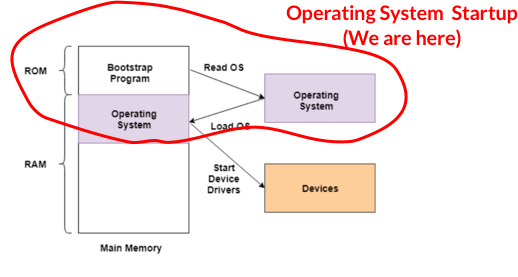
\includegraphics[width=\linewidth]{images/week_2_notes_1_3.png}
        \end{center}


        \begin{itemize}
            \item executes \textbf{Bootstrap Program}
            \begin{itemize}
                \item is the first code that runs when the computer system is started
            \end{itemize}
            \item Entire operating system depnds on the bootstrap program to work
            correctly
            \item Locates and loads kernel (code of operating system) onto RAM
            \begin{itemize}
                \item kernel = code of the operating system
                \item kernel is in HDD
            \end{itemize}
            \item Bootstrap program is in ROM
        \end{itemize}

        \item ROM
        \begin{itemize}
            \item is called \textbf{read-only-memory}
            \item Is also called \textbf{BIOS chip} (Basic Input/Output System)
            \item is non-volatile
            \item is stored in motherboard

            \begin{center}
            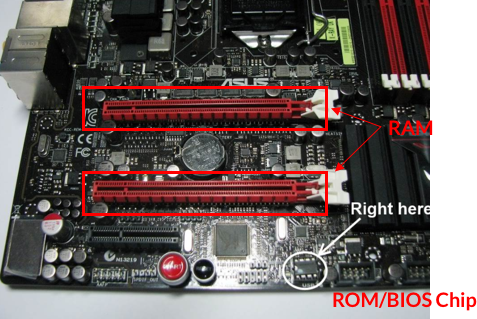
\includegraphics[width=0.8\linewidth]{images/week_2_notes_1_2.png}
            \end{center}
        \end{itemize}
    \end{itemize}

    \item Operating System Startup

    \begin{center}
    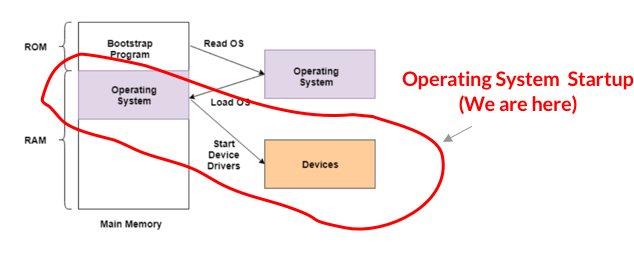
\includegraphics[width=\linewidth]{images/week_2_notes_1_4.png}
    \end{center}

    \begin{itemize}
        \item Initializes OS
        \begin{itemize}
            \item Initialize internal data structures
            \item Create first process
            \item Switch mode to user and start runing first process
            \item Wait for something to happen
        \end{itemize}
    \end{itemize}

    \item Requesting OS Services
    \begin{itemize}
        \item Some services offered by OS are:
        \begin{itemize}
            \item Program execution
            \begin{itemize}
                \item Loading program to memory and executing program
            \end{itemize}
            \item I/O operations
            \begin{itemize}
                \item Keyboard, mouse, speaker
            \end{itemize}
            \item File system manipulation
            \begin{itemize}
                \item Reading and writing files and directories
            \end{itemize}

            \item Error Detection
            \begin{itemize}
                \item Error that pops when printer ink is empty
            \end{itemize}

            \begin{center}
            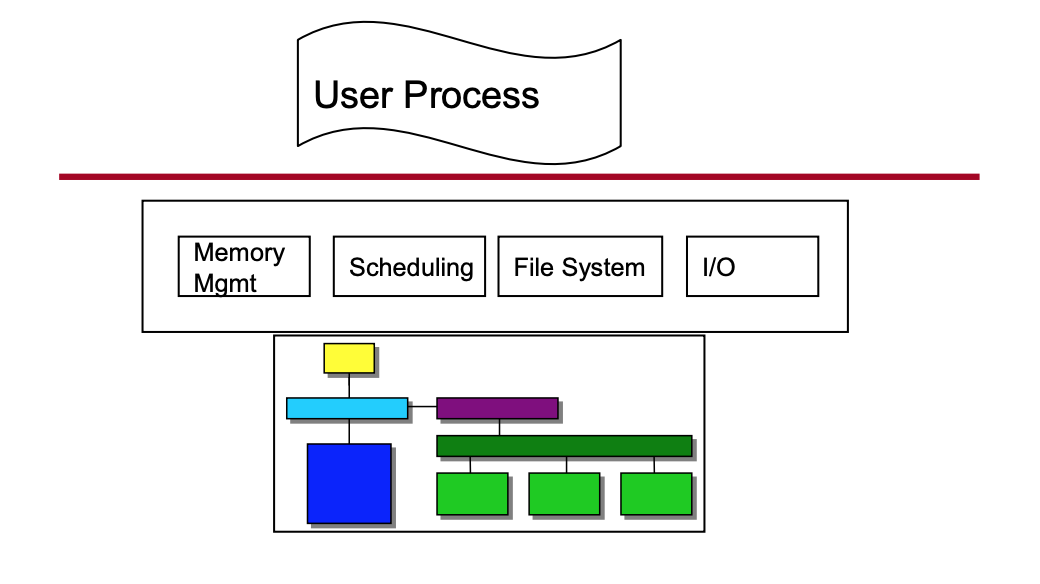
\includegraphics[width=0.7\linewidth]{images/week_2_notes_1_6.png}
            \end{center}
        \end{itemize}

        \item Operating system and user programs are isolated

        \item How do they communicate?
    \end{itemize}
    \item Boundary Crossings

    \bigskip

    \begin{itemize}
        \item Boundary
        \begin{itemize}
            \item Is the line between user applications and kernel
            \item Data is difficult to move back and forth between this line
        \end{itemize}
        \item Boundary Corssings
        \begin{itemize}
            \item Is the communication that occurs between a program and kernel

            \begin{center}
            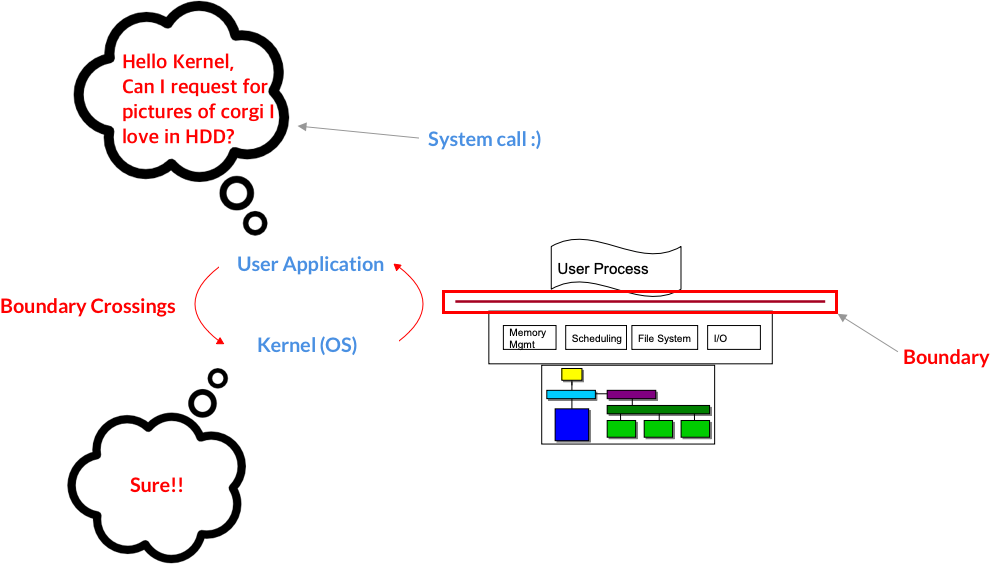
\includegraphics[width=\linewidth]{images/week_2_notes_1_7.png}
            \end{center}

            \item Communication occurs by sending data from one program into kernel,
            and then back
        \end{itemize}
        \item More can be found \href{https://docs.huihoo.com/darwin/kernel-programming-guide/boundaries/chapter_14_section_1.html}{here}
    \end{itemize}

    \item System Calls for Process Management

    \begin{itemize}
        \item Major system calls

        \begin{tabular}{|l|l|}
            \hline
            \textbf{Call} & \textbf{Description}\\
            \hline
            pid = fork() & Create a child process identical to the parent\\
            \hline
            pid = waitpid(pid, \&statloc, options) & Wait for a child to terminate\\
            \hline
            s = execve(name argv, environp) & Replace a process' core image\\
            \hline
            exit(status) & Terminate process execution and return status\\
            \hline
        \end{tabular}
    \end{itemize}

    \bigskip

    \begin{mdframed}
        \begin{itemize}
            \item Wait, System Calls?

            \bigskip

            \textbf{System Calls} are interrupt signals sent by software

            \begin{center}
            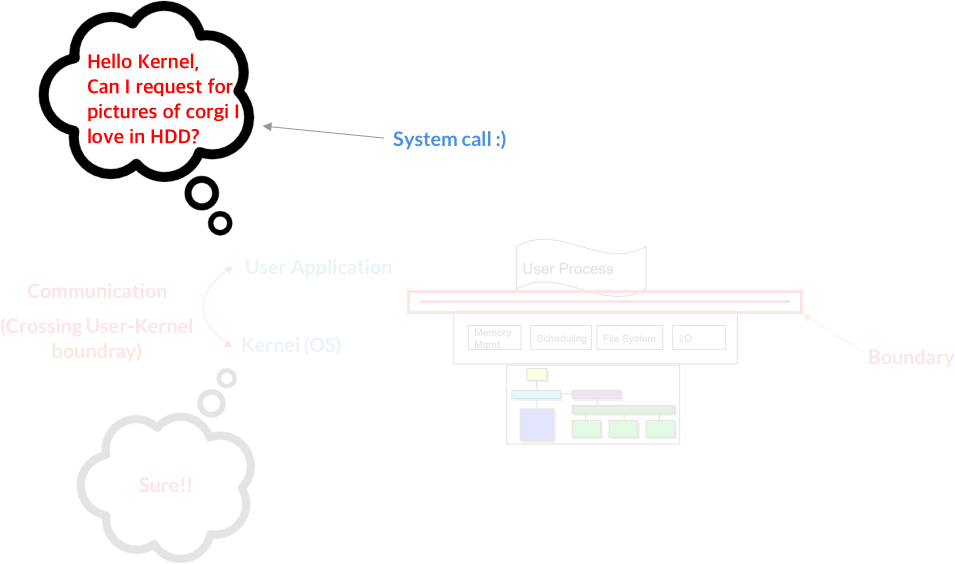
\includegraphics[width=\linewidth]{images/week_2_notes_1_8.png}
            \end{center}

            \begin{itemize}
                \item Is a programmatic way of a program requesting for service to
                kernel of operating system
                \item It's like `Hey OS, could you do $y$? It's really important'
                \item i.e. Fetching a file in hard-disk drive
            \end{itemize}

        \end{itemize}
    \end{mdframed}

    \item System Calls for File Management

    \begin{itemize}
        \item Major system calls

        \begin{tabular}{|l|l|}
            \hline
            \textbf{Call} & \textbf{Description}\\
            \hline
            fd = open(file, how, ...) & Open a file for reading, writing, or both\\
            \hline
            s = close(fd) & Close an open file\\
            \hline
            n = read(fd, buffer, nbytes) & Read data from a file into a buffer\\
            \hline
            n = write(fd, buffer, nbytes) & Write data from a buffer into a file\\
            \hline
            position = lseek(fd, offset, whence) & Move the file pointer\\
            \hline
            s = stat(name, \&buf) & get a file's status information\\
            \hline
        \end{tabular}
    \end{itemize}

    \item System Call Interface
    \begin{itemize}
        \item Interface
        \begin{itemize}
            \item Is a point where two systems, subjects, organizations, etc.
            meet and interact. (Definition)
        \end{itemize}
        \item System Call Interface
        \begin{itemize}
            \item Is the point where user mode and kernel mode meet and interact

            \begin{figure}[h!]
            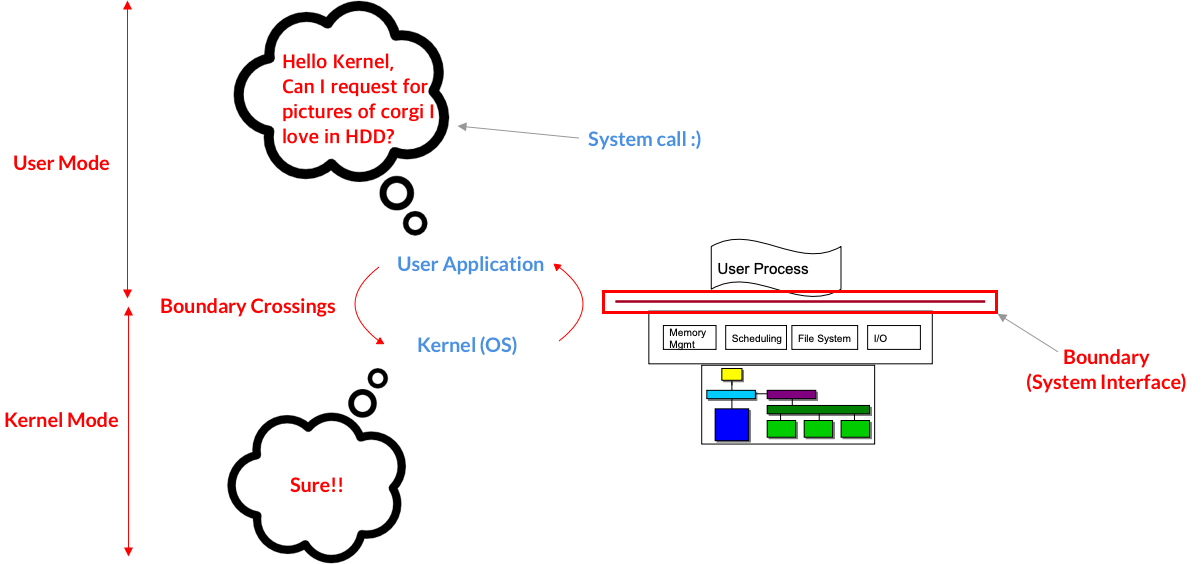
\includegraphics[width=\linewidth]{images/week_2_notes_1_9.png}
            \caption{Now, there really is a party going on here :)}
            \end{figure}

            \item Most of the system call interface are hidden from the programmer
            by API
        \end{itemize}
        \item User Mode
        \begin{itemize}
            \item Cannot directly access memory and other hardwares
            \item Is safe
            \item Crash $\to$ doesn't halt entire system
        \end{itemize}
        \item Kernel Mode
        \begin{itemize}
            \item Does have access to memory and other hardwares
            \item Is a previleged mode
            \item Is not safe
            \item Is fragile
            \item Crash $\to$ halts entire system
            \begin{itemize}
                \item i.e. The Blue Screen of Death \textgreater :)
            \end{itemize}

            \begin{center}
            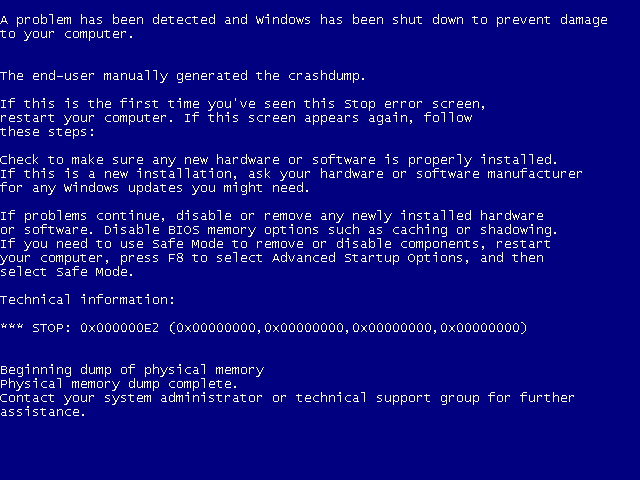
\includegraphics[width=\linewidth]{images/week_2_notes_1_12.png}
            \end{center}
        \end{itemize}

    \end{itemize}
    \item System Call Operation

    \begin{itemize}
        \item Register is a local storage device present in CPU
        \item Register may include the address of the memory location instead of real data
        \item CPU takes data that has to be processed from register

        \begin{center}
        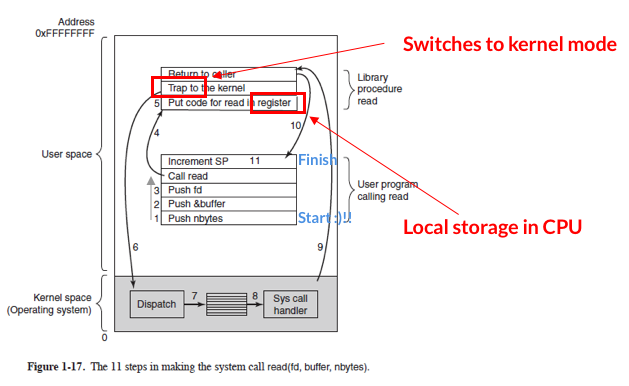
\includegraphics[width=\linewidth]{images/week_2_notes_1_11.png}
        \end{center}

    \end{itemize}

\end{itemize}

\end{document}